% Indicate the main file. Must go at the beginning of the file.
% !TEX root = ../main.tex

%%%%%%%%%%%%%%%%%%%%%%%%%%%%%%%%%%%%%%%%%%%%%%%%%%%%%%%%%%%%%%%%%%%%%%%%%%%%%%%%
% 02_methods
%%%%%%%%%%%%%%%%%%%%%%%%%%%%%%%%%%%%%%%%%%%%%%%%%%%%%%%%%%%%%%%%%%%%%%%%%%%%%%%%

\section{Methods}
\label{methods}

\subsection{Data}%%%%%%%%%%%%%%%%%%%%%%%%%%%%%%%%%%%%%%%%%%%%%%%%%%%%%%%%%%%%%%%

The used data for this project is the SwissImage RS \autocite{swisstopoSWISSIMAGERS2024}
data from the Swiss Federal Office of Topography (SwissTopo).
It is a raster dataset with a resolution of 0.1m containing four bands: RGB and NIR.
In order to cover the area of interest (AOI) 6 tiles of the dataset are needed.
Over this large AOI there are three areas labeled with the corresponding labels \autoref{fig:aoi_labeled}.
These labels were provided by a team of researchers from the ZHAW. The three
areas are distributed over a residential area (83487m\textsuperscript{2}),
an industrial area (132642m\textsuperscript{2}) and a rural area (82740m\textsuperscript{2}).
Two kinds of labels are available: The landcover category \autoref{fig:category_areas} and an assessment of the 
degree of perviousness \autoref{fig:sealed_areas}. In \autoref{fig:label_distribution} the distribution of
the data available for each label is shown for both the landcover category and the sealing assessment.
A third kind of labels was generated by simplifying the degree of perviousness into two classes: pervious and impervious.
This was done by reclassifying the unknown areas to sealed ones since they only consist of BuildingDistortions and
ConstructionSites.

\begin{figure}[H]
    \centering
    \captionsetup{width=0.8\linewidth}
    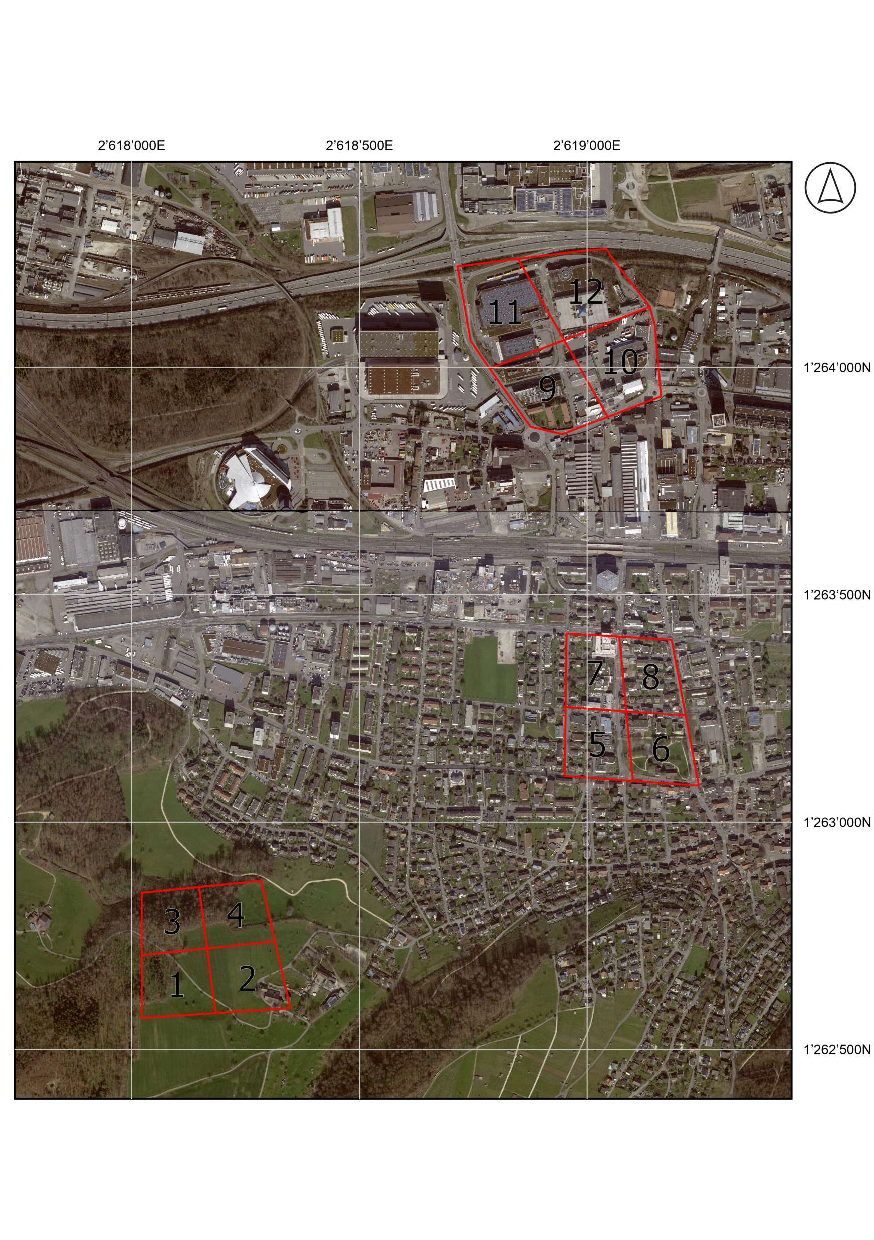
\includegraphics[scale=0.9, trim=-1.1cm 2cm 0cm 2cm, clip]{figures/map_aoi.pdf}
    \caption{Map of the AOI, Pratteln, a  municipality in the canton of Basel-Landschaft, Switzerland. 
    The three marked areas, each split in four tiles, are the areas with corresponding labels. 1 - 4 are in the rural area,
    5 - 8 in the residential area and 9 - 12 in the industrial area.}
    \label{fig:aoi_labeled}
\end{figure}

\begin{figure}[H]
    \centering
    \captionsetup{width=0.8\linewidth}
    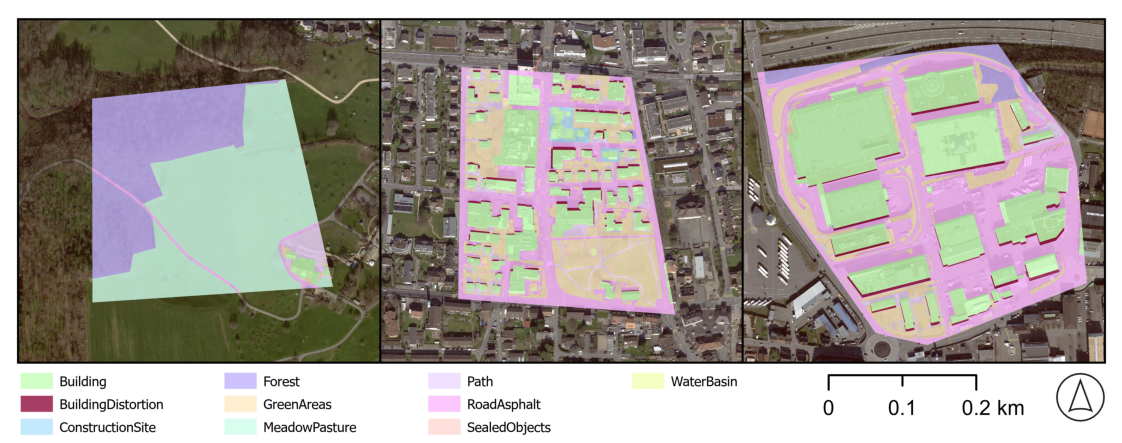
\includegraphics[width=\linewidth]{figures/map_aoi_category.pdf}
    \caption{The three areas with the corresponding landcover categories.}
    \label{fig:category_areas}
\end{figure}

\begin{figure}[H]
    \centering
    \captionsetup{width=0.8\linewidth}
    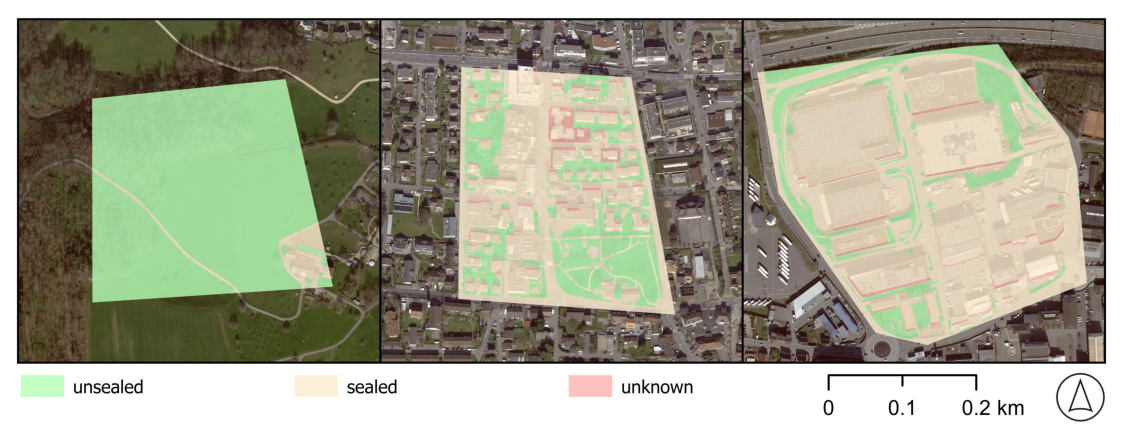
\includegraphics[width=\linewidth]{figures/map_aoi_sealing.pdf}
    \caption{The three areas with the corresponding degree of perviousness.}
    \label{fig:sealed_areas}
\end{figure}

\begin{figure}[H]
    \centering
    \captionsetup{width=0.8\linewidth}
    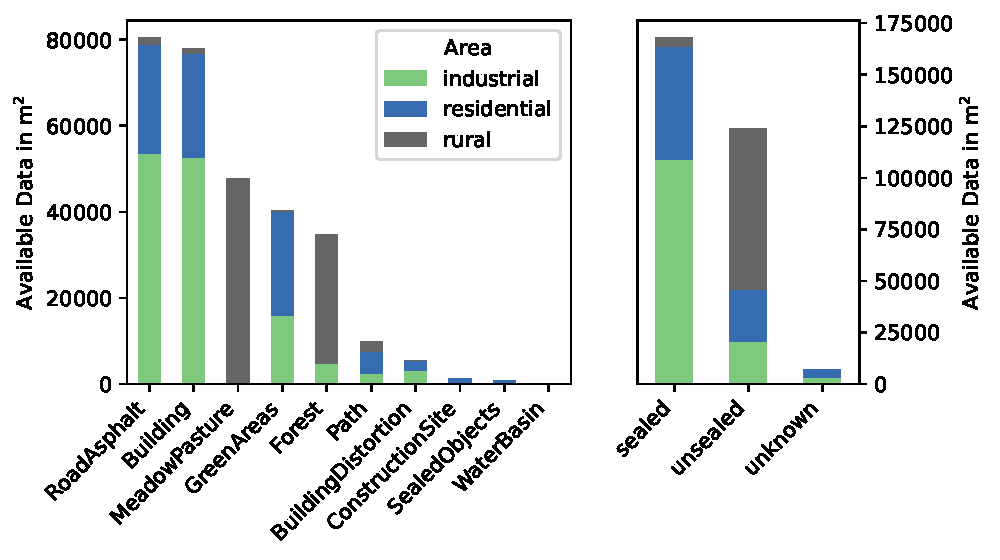
\includegraphics{figures/area_by_category_and_seal.pdf}
    \caption{Available data by label, colored by the area.}
    \label{fig:label_distribution}
\end{figure}


\subsection{Programming Language and Frameworks}%%%%%%%%%%%%%%%%%%%%%%%%%%%%%%%%

To build and train the deep learning model, the programming language Python was used.
The Frameworks PyTorch and Lightning are widely used and powerful tools for building
deep learning models.


\subsection{Model}%%%%%%%%%%%%%%%%%%%%%%%%%%%%%%%%%%%%%%%%%%%%%%%%%%%%%%%%%%%%%%


\subsection{Data Processing and Augmentation}%%%%%%%%%%%%%%%%%%%%%%%%%%%%%%%%%%

To feed data into the neural network, it is necessary to process it into a format that can be used for training.
A standardized sample size is needed to ensure that the model can be trained on the data.


\subsubsection{Preprocessing}%---------------------------------------
In a first step the data was processed using ArcGIS Pro. The process included a few steps implemented as
a model with the Model Builder \autoref{fig:processing_model}. The 6 tiles where mosaicked together and the area of interest 
was clipped. The area labels 1 - 12 and both versions of available data labels where transformed to raster datasets
and added as additional bands to the dataset. The data was then exported as a GeoTIFF file.
In order to use the data in a neural network an additional step was necessary. Using Python,
the data was transformed into Zarr format. This format is a chunked, compressed, N-dimensional array
storage format with multi-scale support. This allows for lazy loading and therefore for a more memory
efficient data access during training.

\begin{figure}[H]
    \centering
    \captionsetup{width=0.8\linewidth}
    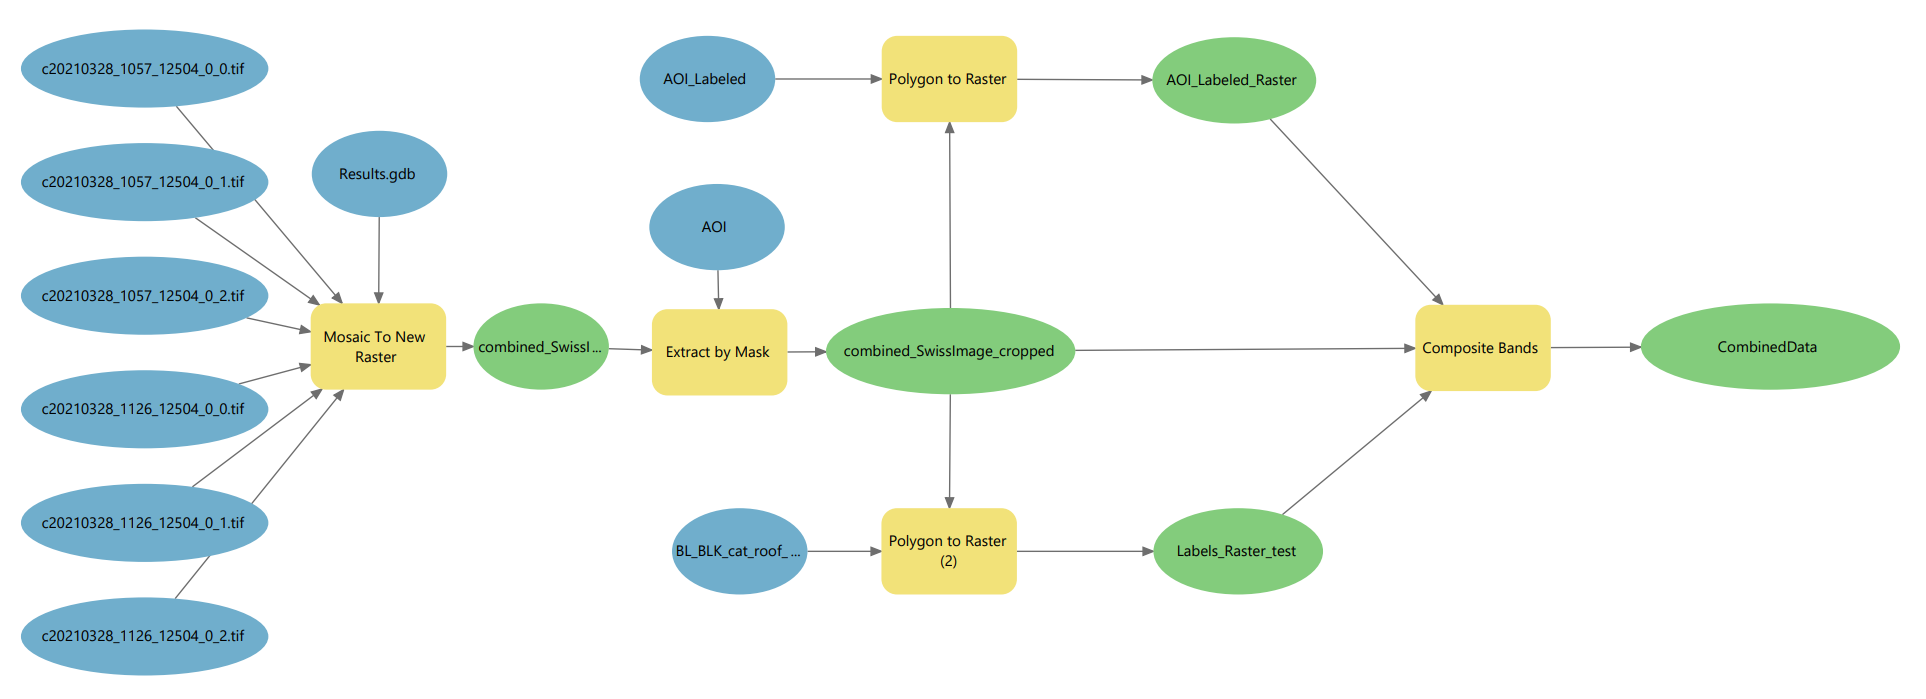
\includegraphics[width=\linewidth]{figures/ArcGIS_Model.png}
    \caption{ArcGIS model used for preprocessing the data.}
    \label{fig:processing_model}
\end{figure}


\subsubsection{Processing and Augmentation}%-------------------------------

To feed the data into a neural network a PyTorch DataLoader was implemented.
The data was sampled as cutouts of size 51x51 pixels, predicting the 5x5 center pixels as output.
This cutout size and output size where implemented as a parameter 
but no other values where tested.
The DataLoader indexes the available data depending on the cutout size and the 
corresponding area labels depending on the purpose - refer to \autoref{tab:areas}. 
It handles the data augmentation on the fly, during training steps.
For the data augmentation a parent class BaseAugmentor was implemented from which the different augmenters inherit. 
The implemented augmentors - refer to \autoref{tab:augmentors} - are then chained into a object of the class AugmentorChain
which can be used in the DataLoader.

\begin{table}[h!]
    \centering
        \begin{tabular}{|l|l|}
        \hline
        \textbf{Category}          & \textbf{Areas}       \\ 
        \hline
        Areas for Training         & 1, 2, 5, 6, 9, 10   \\
        Areas for Validation       & 3, 7, 11            \\
        Areas for Testing          & 4, 8, 12            \\ 
        \hline
        \end{tabular}
    \caption{Division of Areas for Training, Validation, and Testing}
    \label{tab:areas}
\end{table}

\begin{table}[H]
    \centering
        \begin{tabular}{|l|l|}
        \hline
        \textbf{Augmentor} & \textbf{Description} \\
        \hline
        FlipAugmentor & Randomly flips the image vertically and horizontally\\
        RotateAugmentor & Randomly rotates the image 0, 90, 180 or 270° \\
        PixelNoiseAugmentor & Adds random noise to the image (parameter: scale) \\
        ChannelNoiseAugmentor & Adds random noise to the channels (parameter: scale) \\
        \hline
        \end{tabular}
    \caption{Implemented augmentors}
    \label{tab:augmentors}
\end{table}


\subsection{Fitting the Model}%%%%%%%%%%%%%%%%%%%%%%%%%%%%%%%%%%%%%%%%%%%%%%%%%

Fitting the model was done on the IUNR HPC cluster using node 301 a HPE Apollo 6500 Gen10+ 
node running Rocky Linux 8. The node is equipped with 8 NVIDIA L40S GPUs (48GB each), 
dual AMD EPYC 7742 processors, 512 cores, and 5800 GB of storage, 
providing the computational power needed for high-performance tasks.
The training was done using a potential limit of 300 epochs and an early stopping Callback
set to stop after 10 epochs without improvement. The model was trained using the AdamW
optimizer from the PyTorch library. Batch size was set to 128 for training and 256 for validation and prediction.
To calculate the loss the CrossEntropyLoss was used with default parameters and class weights inversely
proportional to the available data per class, in order to give more emphasis to classes with
fewer samples. During training only the best model and the last model where saved.
On completion of the training the best model was loaded and used for prediction on the whole dataset.
This predictions where saved as a Zarr file for later use in the evaluation.
For each the category classification and the perviousness classification two models where trained
with and without data augmentation. The data augmentation was done using the Flip- and RotateAugmentor.
The learning rate was set to 0.001 and weight decay to 0.01.

For the simplified perviousness classification a limited hyperparameter search was done.
All combinations of the following parameters where tested:
\begin{itemize}
    \item Learning rate: 0.001, 0.0001
    \item Weight decay: 0, 0.1, 0.01
    \item Data augmentation: no augmentation, Flip- and RotateAugmentor
\end{itemize}


\subsection{Evaluation}%%%%%%%%%%%%%%%%%%%%%%%%%%%%%%%%%%%%%%%%%%%%%%%%%%%%%%%%

For the performance evaluation of the models, the Python library Scikit-Learn was used \autocite{ScikitlearnMachineLearning}. 
The predictions where loaded from the Zarr file and compared to the ground truth labels.
Accuracy, F1-Score weighted and per class where calculated for every model and stored to a CSV file
for later comparison.